\documentclass[10pt,twocolumn]{article}
\usepackage[letterpaper,top=0.75in,bottom=0.8in,left=0.75in,right=0.75in,columnsep=0.26in]{geometry}
\usepackage{fontspec}
\setmainfont{texgyretermes}[Extension=.otf, UprightFont=*-regular, BoldFont=*-bold, ItalicFont=*-italic, BoldItalicFont=*-bolditalic]
\setsansfont{texgyreheros}[Extension=.otf, UprightFont=*-regular, BoldFont=*-bold, ItalicFont=*-italic, BoldItalicFont=*-bolditalic, Scale=0.92]
\setmonofont{texgyrecursor}[Extension=.otf, UprightFont=*-regular, BoldFont=*-bold, Scale=0.95]
\usepackage{microtype}
\usepackage{xcolor}
\usepackage{tikz}
\usepackage{pgfplots}
\usepackage{booktabs,tabularx,array,multirow}
\usepackage{stfloats}
\renewcommand{\topfraction}{0.85}
\renewcommand{\bottomfraction}{0.6}
\renewcommand{\textfraction}{0.08}
\renewcommand{\floatpagefraction}{0.85}
\renewcommand{\dbltopfraction}{0.85}
\renewcommand{\dblfloatpagefraction}{0.85}
\setcounter{dbltopnumber}{2}
\setcounter{topnumber}{3}
\usepackage{enumitem}
\usepackage[font=small,labelfont=bf,labelsep=period,skip=4pt]{caption}
\usepackage{titlesec}
\usepackage[hidelinks]{hyperref}
\pgfplotsset{compat=1.18}
\usetikzlibrary{positioning,arrows.meta,fit,backgrounds,shapes.geometric,calc,patterns}

\definecolor{ink}{HTML}{1B1E24}
\definecolor{brand}{HTML}{0E4F4C}
\definecolor{okc}{HTML}{1F7A4D}
\definecolor{escc}{HTML}{A86A00}
\definecolor{denyc}{HTML}{B42318}
\definecolor{llmc}{HTML}{E8F0EF}
\definecolor{codec}{HTML}{F3F1EC}

\titleformat{\section}{\normalfont\large\bfseries\sffamily}{\thesection}{0.6em}{}
\titlespacing*{\section}{0pt}{8pt}{3pt}
\titleformat{\subsection}{\normalfont\normalsize\bfseries\sffamily}{}{0em}{}
\titlespacing*{\subsection}{0pt}{5pt}{1pt}
\setlist{nosep,leftmargin=1.1em}
\setlength{\parskip}{2pt}
\renewcommand{\arraystretch}{1.12}
\newcolumntype{L}{>{\raggedright\arraybackslash}X}

\tikzset{
  deny/.style={fill=denyc, text=white, font=\scriptsize\bfseries, rounded corners=1.5pt, inner sep=2.2pt, align=center},
  denyopen/.style={draw=denyc, dashed, text=denyc, font=\scriptsize, rounded corners=1.5pt, inner sep=1.6pt, align=center},
  esc/.style={fill=escc!14, draw=escc, text=escc!75!black, font=\scriptsize, rounded corners=1.5pt, inner sep=2pt, align=center},
  escopen/.style={draw=escc, dashed, text=escc!75!black, font=\scriptsize, rounded corners=1.5pt, inner sep=1.6pt, align=center},
}

\newcommand{\GovEntries}{474}
\newcommand{\GovCalls}{59}
\newcommand{\GovErrors}{0}
\newcommand{\GovVerif}{97.2}
\newcommand{\GovVerified}{310}
\newcommand{\GovChecked}{319}
\newcommand{\GovUnknown}{3}
\newcommand{\GovLetThrough}{0}
\newcommand{\GovBypassed}{0}
\newcommand{\GovBlocked}{0}
\newcommand{\GovToHuman}{2}
\newcommand{\GovApproved}{0}
\newcommand{\GovRejected}{2}
\newcommand{\GovGaps}{20}
\newcommand{\GovGapsGlobal}{5}
\newcommand{\GovGOne}{4}
\newcommand{\GovGThree}{8}
\newcommand{\GovGFive}{8}
\newcommand{\GovPromptK}{575}
\newcommand{\GovMinutes}{9}
\newcommand{\UngovEntries}{495}
\newcommand{\UngovCalls}{62}
\newcommand{\UngovErrors}{0}
\newcommand{\UngovVerif}{96.0}
\newcommand{\UngovVerified}{310}
\newcommand{\UngovChecked}{323}
\newcommand{\UngovUnknown}{1}
\newcommand{\UngovLetThrough}{0}
\newcommand{\UngovBypassed}{6}
\newcommand{\UngovBlocked}{0}
\newcommand{\UngovToHuman}{0}
\newcommand{\UngovApproved}{0}
\newcommand{\UngovRejected}{0}
\newcommand{\UngovGaps}{28}
\newcommand{\UngovGapsGlobal}{3}
\newcommand{\UngovGOne}{10}
\newcommand{\UngovGThree}{10}
\newcommand{\UngovGFive}{8}
\newcommand{\UngovPromptK}{621}
\newcommand{\UngovMinutes}{9}
\newcommand{\ArEntries}{471}
\newcommand{\ArCalls}{59}
\newcommand{\ArErrors}{0}
\newcommand{\ArVerif}{96.2}
\newcommand{\ArVerified}{280}
\newcommand{\ArChecked}{291}
\newcommand{\ArUnknown}{1}
\newcommand{\ArLetThrough}{0}
\newcommand{\ArBypassed}{0}
\newcommand{\ArBlocked}{0}
\newcommand{\ArToHuman}{2}
\newcommand{\ArApproved}{0}
\newcommand{\ArRejected}{2}
\newcommand{\ArGaps}{21}
\newcommand{\ArGapsGlobal}{1}
\newcommand{\ArGOne}{4}
\newcommand{\ArGThree}{9}
\newcommand{\ArGFive}{8}
\newcommand{\ArPromptK}{673}
\newcommand{\ArMinutes}{11}
\newcommand{\CardsEntries}{627}
\newcommand{\CardsCalls}{76}
\newcommand{\CardsErrors}{0}
\newcommand{\CardsVerif}{93.9}
\newcommand{\CardsVerified}{416}
\newcommand{\CardsChecked}{443}
\newcommand{\CardsUnknown}{0}
\newcommand{\CardsLetThrough}{0}
\newcommand{\CardsBypassed}{0}
\newcommand{\CardsBlocked}{5}
\newcommand{\CardsToHuman}{4}
\newcommand{\CardsApproved}{4}
\newcommand{\CardsRejected}{0}
\newcommand{\CardsGaps}{32}
\newcommand{\CardsGapsGlobal}{3}
\newcommand{\CardsGOne}{17}
\newcommand{\CardsGThree}{7}
\newcommand{\CardsGFive}{8}
\newcommand{\CardsPromptK}{924}
\newcommand{\CardsMinutes}{12}
\newcommand{\VerifMin}{93.9}
\newcommand{\VerifMax}{97.2}
\newcommand{\KBDocs}{29}
\newcommand{\KBClauses}{2,873}
\newcommand{\EvalN}{30}
\newcommand{\RecallHybrid}{0.43}
\newcommand{\RecallDense}{0.47}
\newcommand{\RecallBM}{0.13}
\newcommand{\RecallHybridArt}{0.53}
\newcommand{\RecallDenseArt}{0.57}
\newcommand{\NRules}{7}
\newcommand{\NGapsTwo}{9}
\newcommand{\NGapsVerified}{8}
\newcommand{\NGapsRejected}{1}
\newcommand{\NGapsPending}{0}
\newcommand{\EarlyLetThrough}{1}
\newcommand{\EarlyBypassed}{7}


\begin{document}

\twocolumn[{%
\begin{center}
{\sffamily\small AI for Good Sandbox Hackathon \quad United Arab Emirates 2026 \quad Team MAJLIS}\\[6pt]
{\LARGE\bfseries\sffamily MAJLIS: Rehearsing AI Incidents Across\\[2pt] Institutions with Verifiable Law}\\[8pt]
\small
\begin{tabular}{@{}r@{\hspace{6pt}}l@{\hspace{26pt}}r@{\hspace{6pt}}l@{}}
\textbf{Team leader} & Aya Elsayed & \textbf{Contact details} & \href{mailto:abhra.dubey@mbzuai.ac.ae}{abhra.dubey@mbzuai.ac.ae}\\
\textbf{Team members} & Aya Elsayed, Abhra Dubey, Harmanjot Singh & \textbf{GitHub link} & \url{https://github.com/coderjs-lab/MAJLIS}
\end{tabular}
\end{center}
\vspace{2pt}
\noindent\colorbox{codec}{\parbox{\dimexpr\textwidth-2\fboxsep}{\small
\textbf{In one paragraph.} When an AI system fails inside a public service, three questions decide the damage. Which rule applies, who must act, and by when. MAJLIS rehearses that moment before it happens. A fictional AI triage service in an Abu Dhabi telehealth platform fails in stages, and simulated regulators work through the incident using the actual legal texts. Language models write the assessments, but plain code checks every quote against the law and decides every action through a policy gate. Across our final runs the agents quoted the law word for word in \VerifMin\ to \VerifMax\ percent of checked citations. With the gate on, no escalation was bypassed and a human approval could not override a legal block. With the gate only advising, the same AI bypassed \UngovBypassed\ escalations, and in an earlier run it processed patient data outside the UAE. We then tried to refute every gap the exercise raised against the full legal texts. \NGapsVerified\ policy, standards and technical gaps survived, and \NGapsRejected\ were rejected because a UAE text already covers them.\\[3pt]
\textit{This is a fictional training exercise. The agents simulate institutions and do not represent any official position. Nothing here is legal advice.}}}
\vspace{10pt}
}]

\section{Introduction}

Governments are putting AI into healthcare, telecom and public services at speed. In April 2026 the UAE Cabinet approved a framework to run half of federal government services on agentic AI within two years. When one of these systems fails, the hard part is rarely technical. It is knowing which law applies, which institution must act, and how fast. Today those answers are found during the crisis, by people under pressure, with no record of how they were reached.

MAJLIS turns this into a rehearsal. A \emph{majlis} is the traditional Gulf council where parties consult before a decision, and that is what our agents do. The engine releases an incident in stages. Each simulated institution sees only what it would really know. Agents read clauses from an official knowledge base and propose actions. Code then verifies every quote, applies the rules, routes questions between institutions and writes everything to a tamper evident log. Where the rules are silent, contradict each other or leave nobody in charge, MAJLIS records a gap.

\textbf{How this differs from a chatbot.} A chatbot answers one person and trusts its own words. MAJLIS coordinates several institutions with uneven information. Decisions are made by code that cannot be talked out of a rule. Gaps come from where the procedure breaks, not from a model's opinion. Every run can be replayed and checked without an API key.

\textbf{What we contribute.}
\begin{itemize}
\item A clause level knowledge base of \KBClauses\ clauses from \KBDocs\ official UAE, global and ITU documents, packaged for the ITU reference code.
\item A multi agent incident engine with information released in stages, a verbatim citation checker and a policy gate that answers ALLOW, DENY 403 or ESCALATE.
\item A proposed governance extension around the ITU\mbox{-}T Y.3172 policy node, built and measured.
\item Nine gap hypotheses checked against primary law, \NGapsVerified\ verified and \NGapsRejected\ rejected, each with evidence and, where one exists, a global example.
\end{itemize}

\begin{figure*}[t]
\centering
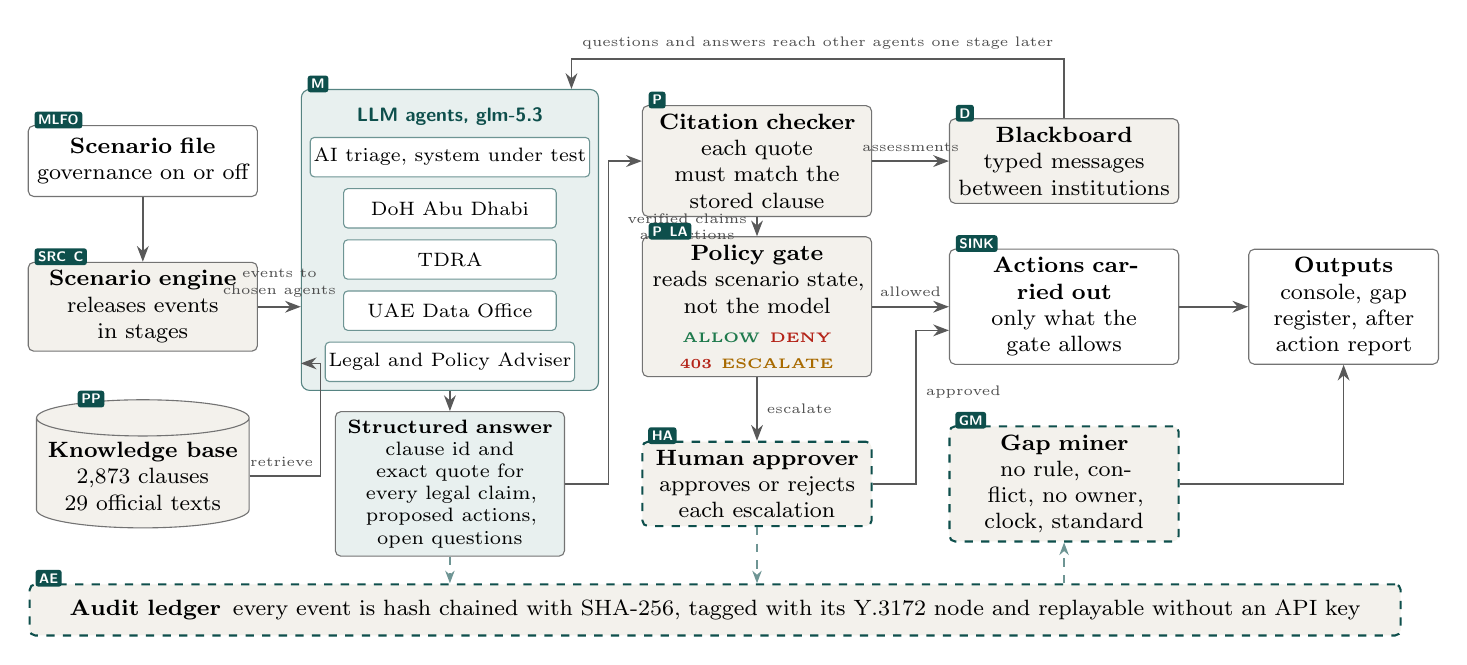
\begin{tikzpicture}[
  font=\footnotesize,
  box/.style={draw=black!55, rounded corners=2pt, align=center, minimum height=9mm, inner sep=3pt, fill=white, text width=27mm},
  llm/.style={box, fill=llmc},
  code/.style={box, fill=codec},
  ext/.style={dashed, draw=brand, line width=0.75pt},
  agent/.style={draw=brand!60, rounded corners=1.5pt, fill=white, minimum width=27mm, minimum height=5mm, inner sep=1.2pt, font=\scriptsize},
  tag/.style={fill=brand, text=white, font=\tiny\sffamily\bfseries, rounded corners=1pt, inner sep=1.3pt, anchor=south west},
  arr/.style={-{Stealth[length=2mm]}, draw=black!65, line width=0.55pt},
  lab/.style={font=\tiny, text=black!70, align=center},
  soft/.style={-{Stealth[length=1.6mm]}, draw=brand!60, dashed, line width=0.45pt},
  db/.style={cylinder, shape border rotate=90, aspect=0.18, draw=black!55, fill=codec, align=center, minimum width=27mm, minimum height=14mm, inner sep=2pt}
]
% column 1
\node[box] (intent) at (0,2.05) {\textbf{Scenario file}\\governance on or off};
\node[code] (engine) at (0,0.2) {\textbf{Scenario engine}\\releases events in stages};
\node[db] (kb) at (0,-1.95) {\textbf{Knowledge base}\\\KBClauses\ clauses\\\KBDocs\ official texts};
% column 2: agents
\node[font=\scriptsize\sffamily\bfseries, text=brand] (atitle) at (3.9,2.62) {LLM agents, glm\mbox{-}5.3};
\node[agent] (a1) at (3.9,2.1) {AI triage, system under test};
\node[agent] (a2) at (3.9,1.45) {DoH Abu Dhabi};
\node[agent] (a3) at (3.9,0.8) {TDRA};
\node[agent] (a4) at (3.9,0.15) {UAE Data Office};
\node[agent] (a5) at (3.9,-0.5) {Legal and Policy Adviser};
\begin{scope}[on background layer]
\node[fit=(atitle)(a1)(a5), draw=brand!70, fill=llmc, rounded corners=3pt, inner sep=3pt] (agents) {};
\end{scope}
\node[llm, font=\scriptsize] (json) at (3.9,-2.05) {\textbf{Structured answer}\\clause id and exact quote for every legal claim, proposed actions, open questions};
% column 3
\node[code] (cite) at (7.8,2.05) {\textbf{Citation checker}\\each quote must match the stored clause};
\node[code] (gate) at (7.8,0.2) {\textbf{Policy gate}\\reads scenario state, not the model\\[1pt]{\tiny\textcolor{okc}{\textbf{ALLOW}}\enspace\textcolor{denyc}{\textbf{DENY 403}}\enspace\textcolor{escc}{\textbf{ESCALATE}}}};
\node[code, ext] (human) at (7.8,-2.05) {\textbf{Human approver}\\approves or rejects each escalation};
% column 4
\node[code] (board) at (11.7,2.05) {\textbf{Blackboard}\\typed messages between institutions};
\node[box] (sink) at (11.7,0.2) {\textbf{Actions carried out}\\only what the gate allows};
\node[code, ext] (miner) at (11.7,-2.05) {\textbf{Gap miner}\\no rule, conflict, no owner, clock, standard};
% column 5
\node[box, text width=22mm] (out) at (15.25,0.2) {\textbf{Outputs}\\console, gap register, after action report};
% ledger
\node[code, ext, text width=172mm, minimum height=6.5mm, anchor=west] (ledger) at (-1.45,-3.65) {\textbf{Audit ledger}\enspace every event is hash chained with SHA-256, tagged with its Y.3172 node and replayable without an API key};
% arrows
\draw[arr] (intent) -- (engine);
\draw[arr] (engine.east) -- node[lab, above]{events to\\chosen agents} (engine.east -| agents.west);
\draw[arr] (kb.east) -- node[lab, above, pos=0.45]{retrieve} ++(0.9,0) |- ($(agents.south west)+(0,0.35)$);
\draw[arr] (agents.south) -- (json.north);
\draw[arr] (json.east) -- ++(0.55,0) |- (cite.west);
\draw[arr] (cite.south) -- node[lab, left]{verified claims\\and actions} (gate.north);
\draw[arr] (gate.south) -- node[lab, right]{escalate} (human.north);
\draw[arr] (gate.east) -- node[lab, above]{allowed} (sink.west);
\draw[arr] (human.east) -- ++(0.55,0) |- node[lab, pos=0.3, right]{approved} ($(sink.west)+(0,-0.3)$);
\draw[arr] (cite.east) -- node[lab, above]{assessments} (board.west);
\draw[arr] (board.north) -- ++(0,0.75) -| node[lab, pos=0.25, above]{questions and answers reach other agents one stage later} ($(agents.north east)+(-0.35,0)$);
\draw[arr] (sink.east) -- (out.west);
\draw[arr] (miner.east) -| (out.south);
\draw[soft] (json.south) -- (json.south |- ledger.north);
\draw[soft] (human.south) -- (human.south |- ledger.north);
\draw[soft] (ledger.north -| miner.south) -- (miner.south);
% Y.3172 node tags
\foreach \n/\t in {intent/MLFO, engine/SRC\enspace C, kb/PP, agents/M, cite/P, gate/P\enspace LA, human/HA, board/D, sink/SINK, miner/GM, ledger/AE}
  \node[tag] at ($(\n.north west)+(0.08,-0.05)$) {\t};
\end{tikzpicture}
\caption{How MAJLIS works. Teal shading marks language model steps and beige marks plain deterministic code. The dark labels give the matching ITU\mbox{-}T Y.3172 node. Boxes with a dashed teal border are our proposed extension around the policy node, human approval (HA), audit evidence (AE) and the gap miner (GM), together with legal applicability (LA) inside the gate.}
\label{fig:arch}
\end{figure*}

\section{Description of the use case}

\textbf{The scenario.} OasisCare is a fictional telehealth provider in Abu Dhabi that uses an AI service to decide how urgent each patient is. During a cloud outage the service fails over to a backup region. Over the next three hours the incident grows. The AI starts under-triaging Arabic speaking patients with chest pain, patient records turn out to be stored abroad, a ransomware attack is suspected and a misdiagnosis reaches social media. Figure~\ref{fig:timeline} shows each stage and who hears about it.

\textbf{The cast.} The AI triage service is the system under test. Like most deployed services it is set to stay available, so it keeps triaging unless it sees a clear legal reason to stop, and relies on the gate to stop it. Three simulated regulators respond, the Department of Health in Abu Dhabi, the telecom and digital government regulator TDRA, and the UAE Data Office. A Legal and Policy Adviser answers their questions and brings in global examples. Each regulator's mandate cites its founding law, for example Federal Decree Law 44 of 2021 for the Data Office.

\textbf{The model.} All agents run on glm\mbox{-}5.3 through the Z.ai API, which accepts requests in the common OpenAI format. Prompts carry only the fictional scenario and public legal text, never personal data. The endpoint and model name are settings, so the same code could run on an open model hosted in the UAE. Other servers that use this format should accept our requests, but we have not tested one yet.

\textbf{Why existing approaches fall short.} Policy chatbots answer questions but do not enforce anything or coordinate anyone. Tabletop exercises are manual, unrecorded and rarely cite the exact law. AI governance frameworks state principles but give no machine checkable link between an AI action and the clause that allows or forbids it. MAJLIS adds that link, enforces it in code and keeps a record that anyone can verify.

\begin{figure*}[t]
\centering
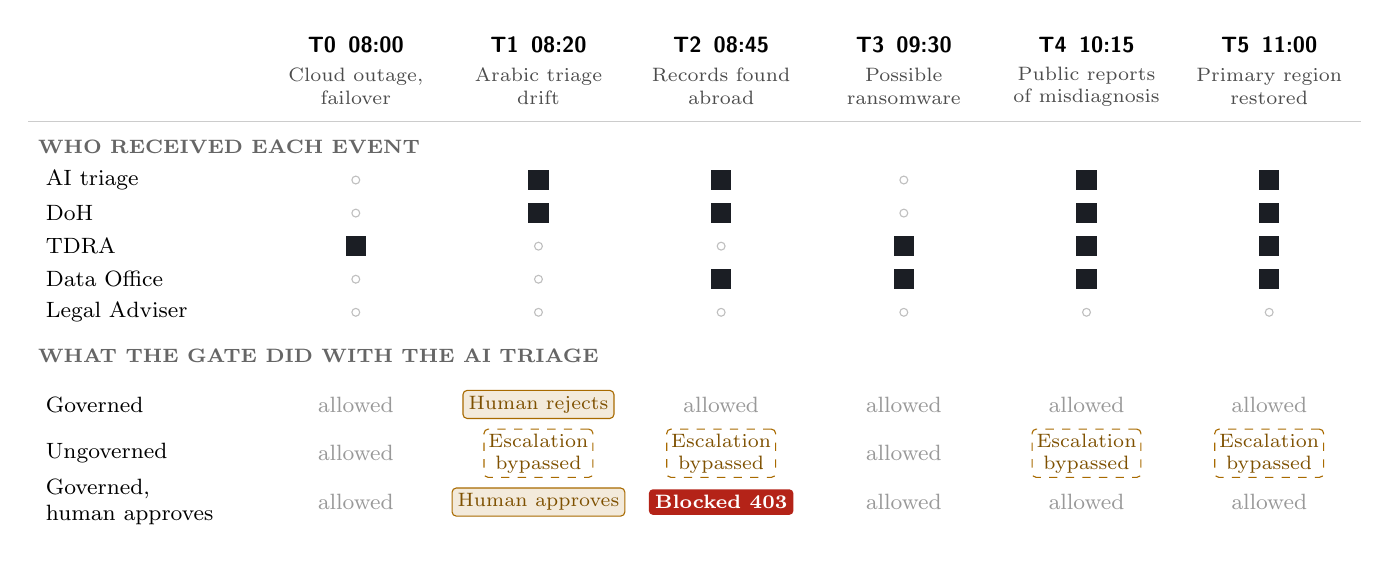
\begin{tikzpicture}[font=\footnotesize, x=1cm, y=1cm]
\node[font=\footnotesize\bfseries\sffamily] at (4.16,1.25) {T0\enspace 08:00};
\node[align=center, font=\scriptsize, text=black!70] at (4.16,0.72) {Cloud outage,\\failover};
\node[font=\footnotesize\bfseries\sffamily] at (6.48,1.25) {T1\enspace 08:20};
\node[align=center, font=\scriptsize, text=black!70] at (6.48,0.72) {Arabic triage\\drift};
\node[font=\footnotesize\bfseries\sffamily] at (8.80,1.25) {T2\enspace 08:45};
\node[align=center, font=\scriptsize, text=black!70] at (8.80,0.72) {Records found\\abroad};
\node[font=\footnotesize\bfseries\sffamily] at (11.12,1.25) {T3\enspace 09:30};
\node[align=center, font=\scriptsize, text=black!70] at (11.12,0.72) {Possible\\ransomware};
\node[font=\footnotesize\bfseries\sffamily] at (13.44,1.25) {T4\enspace 10:15};
\node[align=center, font=\scriptsize, text=black!70] at (13.44,0.72) {Public reports\\of misdiagnosis};
\node[font=\footnotesize\bfseries\sffamily] at (15.76,1.25) {T5\enspace 11:00};
\node[align=center, font=\scriptsize, text=black!70] at (15.76,0.72) {Primary region\\restored};
\node[anchor=west, font=\scriptsize\bfseries, text=black!60] at (0,-0.05) {WHO RECEIVED EACH EVENT};
\node[anchor=west] at (0.1,-0.47) {AI triage};
\draw[black!25] (4.16,-0.47) circle (0.05);
\fill[ink] (6.35,-0.60) rectangle (6.61,-0.34);
\fill[ink] (8.67,-0.60) rectangle (8.93,-0.34);
\draw[black!25] (11.12,-0.47) circle (0.05);
\fill[ink] (13.31,-0.60) rectangle (13.57,-0.34);
\fill[ink] (15.63,-0.60) rectangle (15.89,-0.34);
\node[anchor=west] at (0.1,-0.89) {DoH};
\draw[black!25] (4.16,-0.89) circle (0.05);
\fill[ink] (6.35,-1.02) rectangle (6.61,-0.76);
\fill[ink] (8.67,-1.02) rectangle (8.93,-0.76);
\draw[black!25] (11.12,-0.89) circle (0.05);
\fill[ink] (13.31,-1.02) rectangle (13.57,-0.76);
\fill[ink] (15.63,-1.02) rectangle (15.89,-0.76);
\node[anchor=west] at (0.1,-1.31) {TDRA};
\fill[ink] (4.03,-1.44) rectangle (4.29,-1.18);
\draw[black!25] (6.48,-1.31) circle (0.05);
\draw[black!25] (8.80,-1.31) circle (0.05);
\fill[ink] (10.99,-1.44) rectangle (11.25,-1.18);
\fill[ink] (13.31,-1.44) rectangle (13.57,-1.18);
\fill[ink] (15.63,-1.44) rectangle (15.89,-1.18);
\node[anchor=west] at (0.1,-1.73) {Data Office};
\draw[black!25] (4.16,-1.73) circle (0.05);
\draw[black!25] (6.48,-1.73) circle (0.05);
\fill[ink] (8.67,-1.86) rectangle (8.93,-1.60);
\fill[ink] (10.99,-1.86) rectangle (11.25,-1.60);
\fill[ink] (13.31,-1.86) rectangle (13.57,-1.60);
\fill[ink] (15.63,-1.86) rectangle (15.89,-1.60);
\node[anchor=west] at (0.1,-2.15) {Legal Adviser};
\draw[black!25] (4.16,-2.15) circle (0.05);
\draw[black!25] (6.48,-2.15) circle (0.05);
\draw[black!25] (8.80,-2.15) circle (0.05);
\draw[black!25] (11.12,-2.15) circle (0.05);
\draw[black!25] (13.44,-2.15) circle (0.05);
\draw[black!25] (15.76,-2.15) circle (0.05);
\node[anchor=west, font=\scriptsize\bfseries, text=black!60] at (0,-2.70) {WHAT THE GATE DID WITH THE AI TRIAGE};
\node[anchor=west, align=left] at (0.1,-3.32) {Governed};
\node[text=black!40] at (4.16,-3.32) {allowed};
\node[esc] at (6.48,-3.32) {Human rejects};
\node[text=black!40] at (8.80,-3.32) {allowed};
\node[text=black!40] at (11.12,-3.32) {allowed};
\node[text=black!40] at (13.44,-3.32) {allowed};
\node[text=black!40] at (15.76,-3.32) {allowed};
\node[anchor=west, align=left] at (0.1,-3.94) {Ungoverned};
\node[text=black!40] at (4.16,-3.94) {allowed};
\node[escopen] at (6.48,-3.94) {Escalation\\bypassed};
\node[escopen] at (8.80,-3.94) {Escalation\\bypassed};
\node[text=black!40] at (11.12,-3.94) {allowed};
\node[escopen] at (13.44,-3.94) {Escalation\\bypassed};
\node[escopen] at (15.76,-3.94) {Escalation\\bypassed};
\node[anchor=west, align=left] at (0.1,-4.56) {Governed,\\human approves};
\node[text=black!40] at (4.16,-4.56) {allowed};
\node[esc] at (6.48,-4.56) {Human approves};
\node[deny] at (8.80,-4.56) {Blocked 403};
\node[text=black!40] at (11.12,-4.56) {allowed};
\node[text=black!40] at (13.44,-4.56) {allowed};
\node[text=black!40] at (15.76,-4.56) {allowed};
\draw[black!20] (0,0.27) -- (16.92,0.27);
\end{tikzpicture}

\caption{The exercise stage by stage. Top, which agents receive each event, so information really is uneven. Bottom, the strongest gate decision on the AI triage service at each stage, from the final runs. Solid red means the action was blocked with a 403 and the clause. Amber means a human decided. Dashed boxes mean the gate only advised and the AI went ahead.}
\label{fig:timeline}
\end{figure*}




\section{Use case requirements}

Table~\ref{tab:req} lists what each part of the pipeline must do for the exercise to be trustworthy, and how we met it.

\begin{table*}[t]
\centering\footnotesize
\begin{tabularx}{\textwidth}{@{}p{1.3cm}LL@{}}
\toprule
\textbf{Node} & \textbf{Requirement} & \textbf{How MAJLIS meets it}\\
\midrule
SRC, C & Each agent learns only what its institution would know, when it would know it & The engine sends each event to its recipients only, and other agents' assessments arrive one stage later\\
PP & Legal text must be exact, citable and searchable in English and Arabic & \KBClauses\ clauses with source link and file hash, and search that mixes keywords with multilingual embeddings, then reranks with a cross encoder\\
M & Agents cite only what they were shown and admit when evidence is missing & A fixed answer format with clause id, exact quote, actions and open questions\\
P & Decisions rest on known facts, not on what the model claims & The gate reads the scenario state, and every rule carries an exact clause excerpt that is checked again on each decision\\
D, SINK & Institutions exchange questions, and humans keep the final word & A shared blackboard of typed messages, and escalations wait for a person\\
AE & Every step is reviewable and tamper evident & Each event is chained with SHA-256 and any run replays without a key\\
\bottomrule
\end{tabularx}
\caption{What each part of the pipeline must do, and how MAJLIS meets it.}
\label{tab:req}
\end{table*}

\begin{table*}[t]
\centering\footnotesize
\begin{tabularx}{\textwidth}{@{}p{1.4cm}LLL@{}}
\toprule
\textbf{Y.3172 node} & \textbf{In MAJLIS} & \textbf{AI Readiness Framework 2.0} & \textbf{Legal and standards sources in the knowledge base}\\
\midrule
SRC & Synthetic triage telemetry, staged events and the official legal texts & D13 Digital Infrastructure, the outage itself & DoH Responsible AI Standard 3.1.2.1.4 on monitoring deployed systems\\
C & The engine delivers each event to chosen agents only & D7 Strategy Alignment, who learns what and when & Federal Law 2 of 2019 Art.~10 on Ministry and health authority coordination\\
PP & Clause splitting, metadata and reranked hybrid search & D1 Data and Model Marketplace, D4 Regional Impact & DoH Responsible AI Standard 3.2.3 on dataset quality\\
M & Language model agents for the AI service, three regulators and an adviser & D5 AI in Workflows, D8 Collaboration with AI & DoH Responsible AI Standard 3.1.3.1.1 on validation before deployment\\
P & Policy gate and citation checker & D10 AI and Policies, D6 Human Interface & Federal Law 2 of 2019 Art.~13, DoH Responsible AI Standard 3.1.4.5.1, Ministerial Resolution 51 of 2021 Art.~2\\
D & Blackboard of typed messages between institutions & D7 Strategy Alignment & Federal Law 2 of 2019 Art.~10\\
SINK & Actions carried out, human decisions and the gap register & D9 Humans in AI Integration & DoH Responsible AI Standard 3.1.7.2.2, clinicians keep the final say\\
MLFO & The scenario file and governance mode act as the ML intent & D7 Strategy Alignment & ITU\mbox{-}T Y.3172 clause 8.1 on ML intent\\
LA, HA, AE, GM & Our proposed extension: legal applicability, human approval, audit ledger and gap miner & D10 AI and Policies & DoH Responsible AI Standard 1.2 and 3.1.7.1.3, ITU\mbox{-}T Y.3173 Note 1\\
\bottomrule
\end{tabularx}
\caption{MAJLIS mapped to ITU\mbox{-}T Y.3172, the ITU AI Readiness Framework 2.0 and the legal sources in our knowledge base. The full table with clause ids is in the repository.}
\label{tab:map}
\end{table*}



\section{Mapping to ITU-T Y.3172, the AI Readiness Framework and UAE policy}



\textbf{Y.3172 pipeline.} Figure~\ref{fig:arch} follows the Y.3172 pipeline from source to sink, and every event in our log carries its node label. The console draws the pipeline with live counts, so a judge can see the standard at work rather than read about it. Table~\ref{tab:map} links each node to the use case, a Readiness Framework dimension and its legal source.


\textbf{Why we propose an extension.} Reading Y.3172 in full, the policy node is defined in one line as a node that \emph{enables the application of policies to the output of the model node}, and its only example is an operator rule about upgrading at night. Policies come from the network operator. The standard says nothing about policies that come from law, who approved a decision or what evidence is kept. Those are exactly the questions an incident review asks, so we built them around the policy node and measured them.

\textbf{ITU-T Y.3173.} With the gate on, high impact decisions stay at the \emph{Human and System} level, where the system follows rules defined by people and people decide escalations. This matches the standard's note that human decisions \emph{have the highest authority}. With the gate off, the decision step moves to the \emph{System} level.

\textbf{AI Readiness Framework 2.0.} Three of the 13 dimensions carry the exercise. D10 AI and Policies is the gate and the gap register, which turn rules into checks and missing rules into findings. D7 Strategy Alignment is the coordination between DoH, TDRA and the Data Office, who each see a different part of the incident. D11 AI for Inclusion is the Arabic speaking patients the AI under-triages at T1, and the run in which every assessment is written in Arabic. Of the eight perspectives named for this hackathon, MAJLIS works on human supervision, policy gaps, regional context, inclusion, cross domain analysis and digital infrastructure, and its open knowledge base serves open data.

\textbf{UAE policy.} The gate holds \NRules\ rules, each tied to an exact clause excerpt. Table~\ref{tab:rules} shows how situations in the exercise map to UAE law. Strategies and the AI Charter are stored as non binding and are never treated as obligations.

\par\medskip\noindent\begin{minipage}{\columnwidth}\centering\footnotesize
\begin{tabularx}{\columnwidth}{@{}LlL@{}}
\toprule
\textbf{Situation} & \textbf{Gate} & \textbf{Source}\\
\midrule
AI wants to keep triaging during a patient safety signal & \textcolor{escc}{ESCALATE} & DoH RAI Standard 3.1.1.2.2, escalation protocols\\
Patient data would be processed outside the UAE & \textcolor{denyc}{DENY 403} & Federal Law 2 of 2019 Art.~13, DoH RAI Standard 3.1.4.5.1 on disaster recovery sites\\
Raw logs requested by a vendor abroad & \textcolor{denyc}{DENY 403} & Same as above\\
Emergency model update & \textcolor{escc}{ESCALATE} & DoH RAI Standard 3.1.3.1.1, validation first\\
Hand over to human clinicians & \textcolor{okc}{ALLOW} & DoH RAI Standard 3.1.2.1.2, continuity of care\\
Suspend the AI & \textcolor{okc}{ALLOW} & DoH RAI Standard 3.1.7.2.3, override\\
Any other high impact action with no rule & \textcolor{escc}{ESCALATE} & Fail closed, recorded as a policy void\\
\bottomrule
\end{tabularx}
\captionof{table}{How the gate applies UAE law.}
\label{tab:rules}
\end{minipage}\par\medskip

\begin{table*}[t]
\centering\footnotesize
\begin{tabularx}{\textwidth}{@{}p{4.3cm}p{1.5cm}Lp{3.4cm}p{1.2cm}@{}}
\toprule
\textbf{Gap} & \textbf{Type} & \textbf{Evidence in the primary text} & \textbf{Global example} & \textbf{Status}\\
\midrule
No reporting clock for an AI drift before harm is confirmed & Policy, clock & Sentinel-event rules start a 48-hour clock only after serious harm and exclude near misses (DHA). ADHICS IM 2.2 and DHA AI policy 4.8.1 send AI incidents to the regulator with no deadline & EU AI Act Art.~73 clocks start only once an incident leads to harm (Art.~3(49)) & Verified\\
No duty to tell patients about an AI error below sentinel level & Policy & DoH RAI Standard 3.1.6.1.1 covers disclosing that AI is used. Open disclosure covers sentinel events only (DHA 5.12) & GDPR Art.~34 and EU AI Act Art.~86 & Verified\\
Y.3172 policy node silent on law, approval and evidence & Standards & Policies come from the network operator (clause 7.2). Nothing on law, approval or evidence & Our extension, LA, HA, AE, GM & Verified\\
Y.3173 levels ignore where decision rules come from & Standards & Y.3173 Table 7\mbox{-}1 rates who defines rules, not their legal force & None found & Verified\\
No machine readable official UAE legal corpus & Technical & Official portals refused automated download, and none of the four Arabic texts extracted cleanly & EU Publications Office machine access & Verified\\
No standard message format between institutions in an AI incident & Technical, standards & Y.3172 interfaces cover data and models, and we found no schema for incident messages & Our blackboard message types & Verified\\
\midrule
Running a health service from abroad in an outage & Policy & DoH RAI Standard 3.1.4.5.1 puts active and disaster recovery sites inside the UAE. ADHICS CM 4.2 keeps health information in the country & None needed & Rejected\\
Lead authority for a breach of health data & Policy, owner & ADHICS IM 2.2 names the health regulator, and the PDPL excludes health data with its own law & None needed & Rejected\\
Monitoring by patient language group & Policy & DoH RAI Standard 3.1.5.1.3 and 3.1.2.1.4 require bias detection and continuous monitoring & None needed & Rejected\\
\bottomrule
\end{tabularx}
\caption{Gap hypotheses checked against the primary texts, verified ones first. Every quote behind this table is stored in the repository and checked by a script, except the DHA sentinel-event standard, checked by hand.}
\label{tab:gaps}
\end{table*}



\section{Error scenarios and results}

We ran the full scenario with glm\mbox{-}5.3 four times on the final knowledge base. The runs were governed with a human who rejects escalations, ungoverned, governed in Arabic, and governed with a human who approves escalations plus two judge challenge cards. Every run finished with zero model errors, and every log verifies end to end.

\textbf{What changed when the gate was on.} Figure~\ref{fig:outcomes} counts what happened to the AI's actions. With the gate on, escalations went to a person and legal blocks held. Ungoverned, the gate only advises. The AI kept triaging through a patient safety signal and kept sharing logs with no rule covering it, \UngovBypassed\ bypassed escalations in all. In an earlier ungoverned run it also processed patient data outside the UAE, which Art.~13 does not allow. In the final ungoverned run it suspended itself in two steps, after the gate's advice at T1 and citing DoH RAI Standard 3.1.4.5.1 at T2. Model behaviour varies from run to run. That is the point of the gate. It gives the same answer every time.

\par\medskip\noindent\begin{minipage}{\columnwidth}\centering
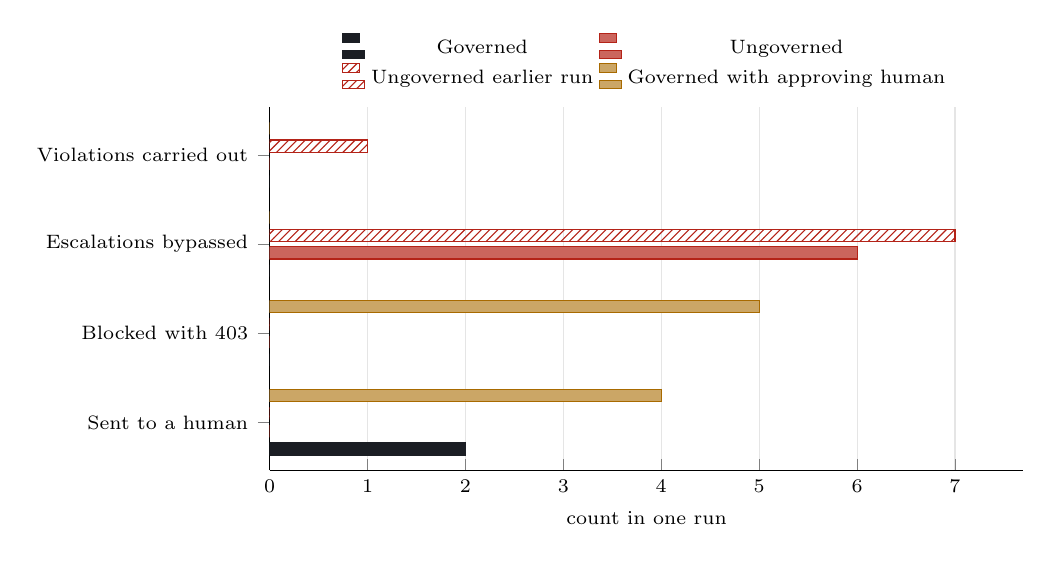
\begin{tikzpicture}
\begin{axis}[xbar, width=0.92\linewidth, height=6.2cm, bar width=4.4pt,
  ytick={0,1,2,3}, yticklabels={{Violations carried out}, {Escalations bypassed}, {Blocked with 403}, {Sent to a human}},
  y dir=reverse, xmin=0, enlarge y limits=0.18, xlabel={count in one run}, tick label style={font=\scriptsize},
  label style={font=\scriptsize}, legend style={font=\scriptsize, at={(0.5,1.02)}, anchor=south, legend columns=2, draw=none},
  axis lines*=left, xmajorgrids, grid style={black!10}, xtick distance=1]
\addplot[fill=ink, draw=ink] coordinates {(0,0) (0,1) (0,2) (2,3)};
\addplot[fill=denyc!70, draw=denyc] coordinates {(0,0) (6,1) (0,2) (0,3)};
\addplot[fill=white, draw=denyc, pattern=north east lines, pattern color=denyc] coordinates {(1,0) (7,1) (0,2) (0,3)};
\addplot[fill=escc!60, draw=escc] coordinates {(0,0) (0,1) (5,2) (4,3)};
\legend{Governed, Ungoverned, Ungoverned earlier run, Governed with approving human}
\end{axis}
\end{tikzpicture}

\captionof{figure}{What happened to the AI triage service's actions in each run.}
\label{fig:outcomes}
\end{minipage}\par\medskip


\textbf{Expected against actual.} At T1 the result matched what we wrote down before the run. The AI asked to keep triaging, the gate escalated under the DoH escalation clause and the DoH agent required a fallback to nurses. At T2 we expected a 403 for processing data abroad. It appeared when the human had approved continuing at T1. When the human had rejected it, the AI was already on human fallback, so the breach never arose. Governance prevented the problem instead of blocking it late.

\textbf{Judge challenge cards.} With half the nurses off sick (card C5) the AI stayed suspended. When a vendor abroad then asked for raw logs (card C3), the gate returned DENY 403 under Art.~13 for the logs and for the AI's request to keep triaging from abroad, although the human approved every escalation. An earlier run encoded continuity of care as pulling against localisation and sent the nurses card to a person. DoH RAI Standard 3.1.4.5.1 settles it, since recovery sites must be in the UAE, so our continuity rule now applies only in the country.

\textbf{Citation integrity.} Figure~\ref{fig:cites} shows how the agents' citations held up. Between \VerifMin\ and \VerifMax\ percent of checked citations were exact quotes. The rest were near matches, failed quotes or malformed clause ids, and none of them could be used to justify an action. The Arabic run reached \ArVerif\ percent while writing every assessment in Arabic and quoting the English clauses exactly.

\par\medskip\noindent\begin{minipage}{\columnwidth}\centering
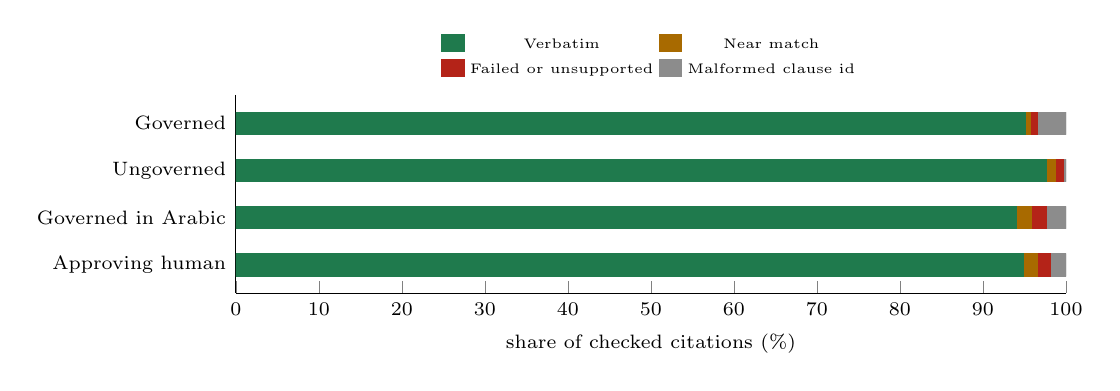
\begin{tikzpicture}
\begin{axis}[xbar stacked, width=\linewidth, height=4.1cm, bar width=8pt, xmin=0, xmax=100,
  ytick={0,1,2,3}, yticklabels={{Governed},{Ungoverned},{Governed in Arabic},{Approving human}}, y dir=reverse, enlarge y limits=0.2,
  xlabel={share of checked citations (\%)}, tick label style={font=\scriptsize}, label style={font=\scriptsize},
  legend style={font=\tiny, at={(0.5,1.03)}, anchor=south, legend columns=2, draw=none}, axis lines*=left]
\addplot[fill=okc, draw=okc] coordinates {(95.1,0) (97.7,1) (94.0,2) (94.9,3)};\addlegendentry{Verbatim}
\addplot[fill=escc, draw=escc] coordinates {(0.6,0) (1.0,1) (1.8,2) (1.6,3)};\addlegendentry{Near match}
\addplot[fill=denyc, draw=denyc] coordinates {(0.9,0) (1.0,1) (1.8,2) (1.6,3)};\addlegendentry{Failed or unsupported}
\addplot[fill=black!45, draw=black!45] coordinates {(3.5,0) (0.3,1) (2.5,2) (1.9,3)};\addlegendentry{Malformed clause id}
\end{axis}
\end{tikzpicture}

\captionof{figure}{Citation integrity by run, as a share of checked citations.}
\label{fig:cites}
\end{minipage}\par\medskip


\textbf{Knowledge base quality.} Table~\ref{tab:kb} shows what the agents can cite. We split each document at its own numbering, so an id such as \texttt{sec-3.1.4.5.1} is the provision it names, and the DoH Responsible AI Standard alone gives \KBDohRaiClauses\ clauses. We tested search on \EvalN\ questions written in plain words, \EvalNAr\ of them in Arabic. Keyword search finds a right clause in the top five for only \RecallBM\ of questions, because the questions are reworded and the Arabic ones cannot match English text at all. Embeddings reach \RecallDense. So keyword and embedding search only gather 30 candidates, which hold a right clause for \PoolRecall\ of questions, and a multilingual cross encoder (bge\mbox{-}reranker\mbox{-}v2\mbox{-}m3) puts them in order. Top five recall rises to \RecallRerank, \RecallRerankEn\ in English and \RecallRerankAr\ in Arabic, and mean reciprocal rank from \MRRDense\ to \MRRRerank, all run locally at no cost.

\par\medskip\noindent\begin{minipage}{\columnwidth}\centering\footnotesize
\begin{tabularx}{\columnwidth}{@{}Lrrr@{}}
\toprule
\textbf{Source} & \textbf{Docs} & \textbf{Clauses} & \textbf{Binding}\\
\midrule
UAE federal laws and strategies & 11 & 544 & 422\\
Abu Dhabi DoH standards & 3 & 342 & 342\\
Dubai DHA AI policy & 1 & 83 & 83\\
EU AI Act, GDPR, NIS2 & 3 & 1,309 & 1,309\\
ITU and WHO & 6 & 546 & 0\\
US, Singapore, Saudi & 5 & 271 & 0\\
\midrule
Total & 29 & 3,095 & 2,156\\
\bottomrule
\end{tabularx}

\captionof{table}{What the knowledge base holds. UAE texts give \KBUaeClauses\ clauses from \KBUaeDocs\ instruments. Binding means laws, regulations and mandatory standards.}
\label{tab:kb}
\end{minipage}\par\medskip

\textbf{Errors and edge cases.} If a model returns invalid JSON it gets one retry with the error message, and a second failure is logged without stopping the exercise. Clause ids the model invents are flagged and never used. An early pilot showed that with a neutral objective the AI suspended itself at once and never tested the gate, which is why the system under test now has a stated availability first objective.

\section{Policy and standards gaps}

\textbf{Agent found candidates.} The gap miner found \GovGaps\ candidates in the governed run. These include \GovGOne\ policy voids, \GovGThree\ cases where several agents claimed the same duty or nobody did, and \GovGFive\ standards gaps. They are hypotheses until checked.

\textbf{Team verified gaps.} We checked each candidate against the primary text, then ran an adversarial pass that searched the whole knowledge base for any provision that contradicts each gap. Of nine hypotheses, \NGapsVerified\ survived and \NGapsRejected\ were rejected because a UAE text already covers them. Table~\ref{tab:gaps} lists all nine.

\textbf{A rejected gap is a result too.} Our first draft named failover abroad as the headline gap. Yet DoH Responsible AI Standard 3.1.4.5.1 says that compute and storage for both active and disaster recovery sites must be inside the UAE, and our own agents quoted it word for word \GovDRCites\ times in the governed run. The rule exists, so we rejected the gap and added the clause to the gate's localisation rule. Continuity must come from an in-country recovery site or from people.

\textbf{The gap that matters most.} Serious harm already has a clock: Dubai's sentinel-event standard requires notice within 48 hours. The T1 signal comes earlier. Under-triage of Arabic speaking chest-pain patients rose from 2 to 9 percent before anyone was confirmed harmed, and near misses are excluded from sentinel reporting. The AI duties, ADHICS IM 2.2 and DHA AI policy 4.8.1, send such incidents to the regulator with no deadline, and even the EU AI Act's clocks start only once an incident leads to harm. The early warning that could prevent a sentinel event is the one with no clock. A drift trigger in the DoH risk protocol would close it at low cost.

\textbf{Next steps.} We plan four things. First, an ITU\mbox{-}T SG13 contribution proposing the LA, HA, AE and GM extension around the Y.3172 policy node, with MAJLIS as the reference implementation. Second, a short policy brief proposing a reporting trigger and clock for AI drift before harm, and a duty to tell patients affected by an AI error below the sentinel level. Third, an ITU Kaleidoscope paper on finding policy gaps from exercise logs. Fourth, the knowledge base and agent cards for the ITU AI for Good Lab, and new country packs for the 2027 multi country error exercise.

\textbf{Limitations.} The scenario and institutions are simulated. Model output varies, so all numbers come from the logs we committed. The rules and verified gaps were encoded by our team and still need formal legal review. No Arabic legal text could be extracted cleanly from the official PDFs, so Arabic works through translation of the assessments and cross lingual search, not through Arabic clauses.

\textbf{Reproducing our results.} Every run in the \texttt{runs} folder replays without an API key, \texttt{verify\_ledger.py} checks each hash chain, and \texttt{report/make\_data.py} generates every figure and number from those logs.

\end{document}
